%%% In this section, you will describe all of the various artifacts that you will generate and maintain during the project life cycle. Describe the purpose of each item below, how the content will be generated, where it will be stored, how often it will be updated, etc. Replace the default text for each section with your own description. Reword this paragraph as appropriate.

\subsection{Major Documentation Deliverables}
\subsubsection{Project Charter}
The project charter is intended to communicate Team UR5's understanding and research on the project. It is the current list of commitments the team will be making. The initial version of the document will be delivered October 3, 2022. The final version will be delivered during the second semester in May 2023. This document will be maintained and updated after every sprint as needed, and when the sponsor approves of these changes.

% Describe how this document will be maintained and updated (how often, under what circumstances, etc.). When will the initial version be delivered? When will the final version be delivered?
https://www.overleaf.com/project/631b8af69f1ea6c375d502b0
\subsubsection{System Requirements Specification}
The Systems Requirements Specification will be maintained and updated during every sprint as features are added or with further understanding of the technology. The initial version of this document will be delivered October 24, 2022. The final version will be delivered during the second semester in May 2023.

% Describe how this document will be maintained and updated (how often, under what circumstances, etc.). When will the initial version be delivered? When will the final version be delivered?

\subsubsection{Architectural Design Specification}
The Architectural Design Specification will be maintained and updated as needed during every sprint especially when there are changes in design or clarifications. The initial version of this document will be delivered November 14, 2022. The final version will be delivered during the second semester in May 2023.

% Describe how this document will be maintained and updated (how often, under what circumstances, etc.). When will the initial version be delivered? When will the final version be delivered?

\subsubsection{Detailed Design Specification}
The Detailed Design Specification will be maintained and updated as needed during every sprint especially when there are changes in design or clarifications. The initial version of this document will be delivered within the first quarter of 2023. The final version will be delivered during the second semester in May 2023.

% Describe how this document will be maintained and updated (how often, under what circumstances, etc.). When will the initial version be delivered? When will the final version be delivered?

\subsection{Recurring Sprint Items}
\subsubsection{Product Backlog}
Items will be added to the product backlog as the System Requirements Specification document is updated. These items will be prioritized based on customer needs and feasibility of the requirement for the current point in time. Team vote and feedback will also be taken into consideration. Jira Software by Atlassian will be used to maintain and work collaboratively on the product backlog.

% How will items be added to the product backlog from the SRS? How will these items be prioritized? Who makes the decision (product owner, group vote, etc.)? What software will be used to maintain and share the product backlog with team members and stakeholders?

\subsubsection{Sprint Planning}
Each sprint will be planned based on documentation and feature implementation deadlines. Team meetings will be held after each sprint to determine the sprint goals. There will be 4 sprints for the first semester and 4 sprints for the second semester, totalling 8 sprints for both semesters.

% How will each sprint plan be planned? How many sprints will there be (you need to look at the schedules for this course and previous Senior Design II courses during the appropriate semesters to figure this out).

\subsubsection{Sprint Goal}
The team will meet and discuss sprint goals. These sprint goals will be decide as a team. Our customer Christopher McMurrough will be involved in the process as needed through scheduled meetings.

% Who decides the sprint goal? How will you involve your customer in this process?

\subsubsection{Sprint Backlog}
Team discussion will be held to determine which product backlog items will make their way into the sprint backlog. The backlog will be maintained using Jira Software developed by Atlassian.

% Who decides which product backlog items make their way into the sprint backlog? How will the backlog be maintained (collaboration software, a "scrum board", etc.)?

\subsubsection{Task Breakdown}
Each team member will voluntarily claim a task, otherwise it will be random. Time spent on tasks will be documented using Jira Software.

% How will individual tasks be assigned from the sprint backlog? Will it be up to each team member to voluntarily claim a task, or will it come from the product owner? How will time spent on tasks be documented?

\subsubsection{Sprint Burn Down Charts}
The burn down charts will allow the team to track the progress of the project. Currently, using Jira Software will automatically generate the burn down charts for each sprint. Each individual team member is responsible for manually updating the effort and time spent as they complete each assigned task. Jira Software will also be able to access all of this. In addition to the Jira log, Microsoft Excel will be used to manually create the burn down charts in case members don't update on Jira. See Figure 2 and 3 for examples.

\begin{figure}[h!]
    \centering
    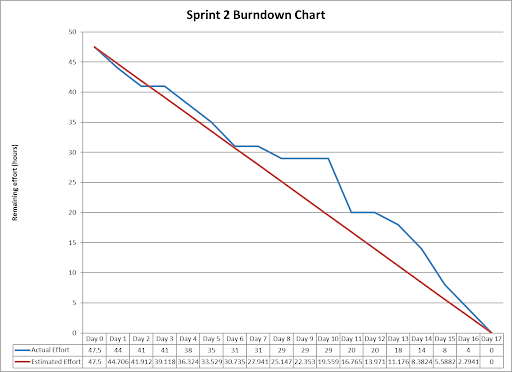
\includegraphics[width=1.0\textwidth]{images/burndown.png}
    \caption{Example sprint burn down chart}
\end{figure}

\begin{figure}[h!]
    \centering
    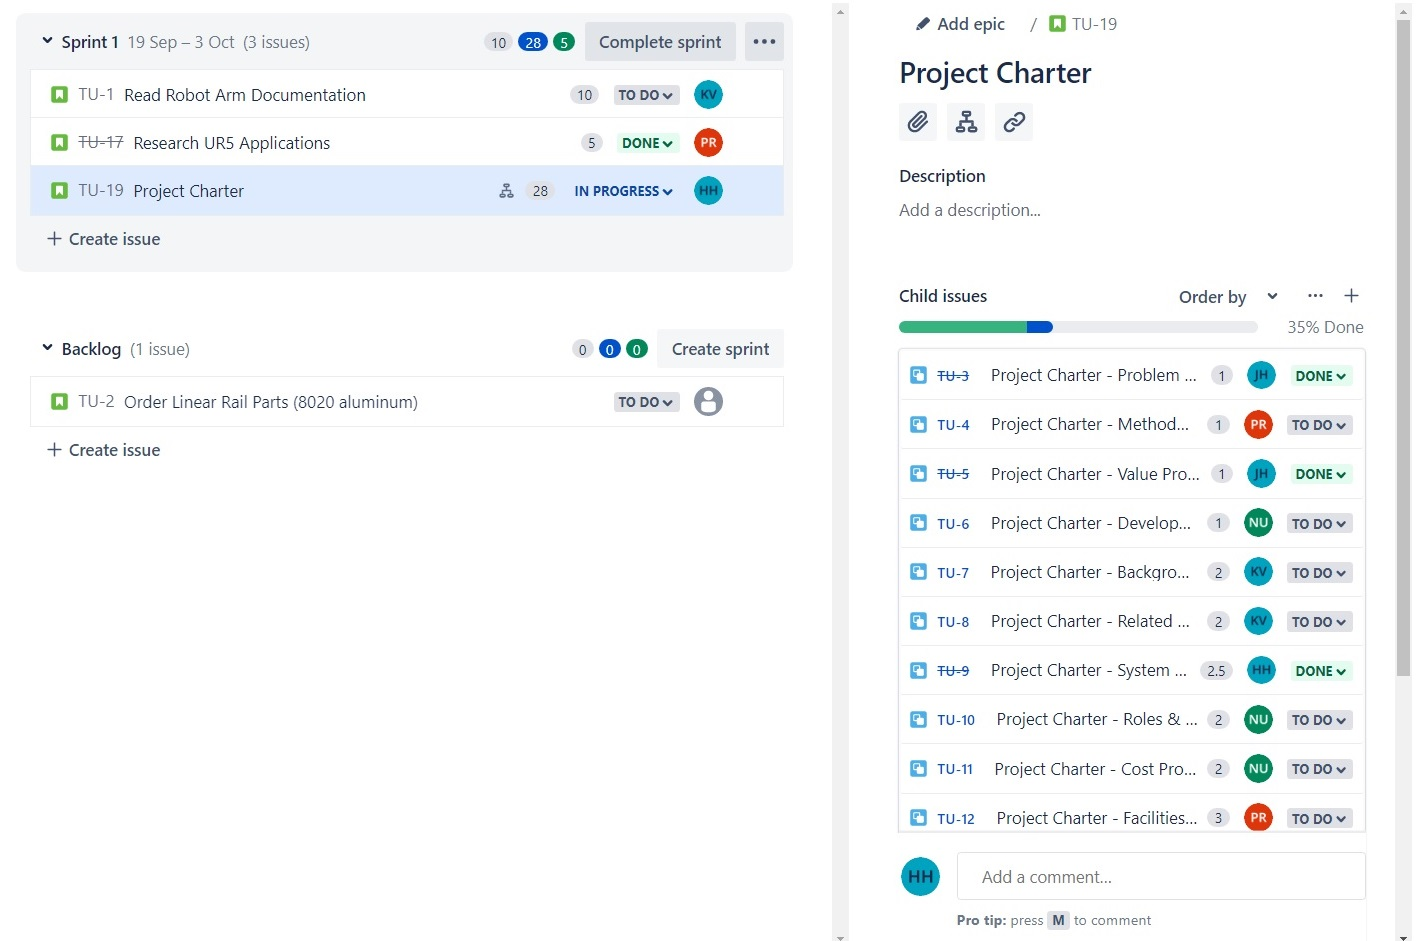
\includegraphics[width=1.0\textwidth]{images/sprint-burndown-tasks.jpg}
    \caption{Example task tracking}
\end{figure}

% Who will be responsible for generating the burn down charts for each sprint? How will they be able to access the total amount of effort expended by each individual team member? What format will the burn down chart use (include an example burn down chart below).

\subsubsection{Sprint Retrospective}
The sprint retrospective will be handled as a team during team meetings. This discussion will happen after each sprint review presentation at the end of each sprint. What went well, and what is needed to be adjusted will be documented as a team before the next sprint plan meeting.

% How will the sprint retrospective be handled as a team? When will this discussion happen after each sprint? What will be documented as a group and as individuals, and when will it be due?

\subsubsection{Individual Status Reports}
Each individual member will primarily report the tasks assigned to them and the time spent on each task for each sprint. Individuals can also include in their report any concerns or issues that may be addressed for future sprints.

% What sort of status will be reported by each individual member, and how often will it be reported? What key items will be contained in the report?

\subsubsection{Engineering Notebooks}
%%% notes, status reports, budgeting, sprint info
% The engineering notebook may contain any project notes, status reports, budgeting, sprint information, etc. It will be updated every week by each team member at minimum. The minimum amount of pages that will be completed will be 1 page for each sprint period. These sprint periods are around 2 weeks long. Any team member that is not the author will sign as a "witness" for each page.

% How often will the engineering notebook be updated, at a minimum, by each team member? What is the minimum amount of pages that will be completed for each interval, and how long will that interval be? How will the team keep each member accountable? Who will sign of as a "witness" for each ENB page?

\subsection{Closeout Materials}
\subsubsection{System Prototype}
Included in the final system prototype will be all major components (computer software, UR5, sensors, checkerboard, etc.) to demonstrate a game with the UR5.

% What will be included in the final system prototype? How and when will this be demonstrated? Will there be a Prototype Acceptance Test (PAT) with your customer? Will anything be demonstrated off-site? If so, will there be a Field Acceptance Test (FAT)?

\subsubsection{Project Poster}
Included on the project poster will be an overview, methodology and design, and results. Poster dimensions will be 32 inches tall by 40 inches wide.

% What will be included on the poster, what will be the final dimensions, and when will it be delivered?

% \subsubsection{Web Page}
% The project web page will have the project's overview, design, results, and document deliverables. The web page will be accessible to the public. When the web page will be delivered and updated is still to be decided.

% What will be included on the project web page? Will it be accessible to the public? When will this be delivered? Will it be updated throughout the project, or just provided at closeout (at a minimum, you need to provide a simple web page at the end).

\subsubsection{Demo Video}
Shown in the demo video will be the robot playing a game with a human. B-reel footage will be recorded throughout project implementation to show progress and different features.

% What will be shown in the demo video(s)? Will you include a B-reel footage for future video cuts? Approximately how long will the video(s) be, and what topics will be covered?

\subsubsection{Source Code}
The source code will be maintained on GitHub using the Git version control system. The source code will also be publicly available to the customer through GitHub. License terms are still to be decided, but still likely be listed in a single ReadMe file.

% How will your source code be maintained? What version control system will you adopt? Will source code be provided to the customer, or binaries only? If source code is provided, how will it be turned over to the customer? Will the project be open sourced to the general public? If so, what are the license terms (GNU, GPL, MIT, etc.). Where will the license terms be listed (in each source file, in a single readme file, etc.).

\subsubsection{Source Code Documentation}

The team plans to write a README for documentation and setup instructions for future users. The team also plans to potentially look into using Doxygen or Pydocs to generate the documentation. The format of the final documentation is still to be decided, however it is likely it will provided as a PDF or HTML file.

% The team plans to look into using Doxygen or Pydocs to generate the documentation. The format of the final documentation is still to be decided, however it is likely it will provided as a PDF or HTML file.

% What documentation standards will be employed? Will you use tools to generate the documentation (Doxygen, Javadocs, etc.). In what format will the final documentation be provided (PDF, browsable HTML, etc.)?

\subsubsection{Hardware Schematics}
The project will involve the UR5 Robot Arm. This robot arm will need a gripper for picking up pieces. In addition to that, a camera will be needed for the robot to detect the state of the game board, determine its next move, and move its pieces. The rest of the project involves python scripts.

% Will you be creating printed circuit boards (PCBs) or wiring components together? If so, list each applicable schematic and what sort of data it will contain (PCB layout, wiring diagram, etc.). If your project is purely software, omit this section.

\subsubsection{CAD files}
The project will need custom checker pieces if the UR5 plans to use a magnetic gripper to pick up the pieces. The FabLab at UTA has software support for SketchUp, Meshmixer, Tinkercad, Fusion 360, and SolidWorks. Currently, the plan is to use the free, online 3D modeling program Tinkercad to make the pieces. Blender could also be another free option to use outside of the software supported in the FabLab. The CAD files will be saved in STL file format to work with the 3D printers available in the FabLab at UTA.

% Will the project involve any mechanical design, such as 3D printed or laser-cut parts? If so, what software will you use to generate the files and what file formats will you provide in your closeout materials (STL, STEP, OBJ, etc.). If your project is purely software, omit this section.

\subsubsection{Installation Scripts}
There are currently no plans to provide installation scripts. At the moment, instructions are planned to be found in the ReadMe file on the GitHub repository.

% How will the customer deploy software to new installations? Will you provide installation scripts, install programs, or any other tools to improve the process? Will there be multiple scripts provided (perhaps separate scripts for the graphical front end and back end server software)? 

% \subsubsection{User Manual}
% A digital user manual will be provided for the customer. This digital user manual can also be printed.

% Will you customer need a printed or digital user manual? Will they need a setup video? Decide now what will be provided and discuss.